%amsart class
\documentclass[a4paper, 10pt, reqno]{amsart}

%Packages
\usepackage[utf8]{inputenc}
\usepackage[english]{babel}
\usepackage{graphics}
\usepackage{physics}
\usepackage{listings}
\usepackage{hyperref}
\usepackage{blindtext}
\usepackage{xcolor}
\usepackage{subcaption}
\usepackage{pgf}
\usepackage{tikz}
\usepackage{tikzscale}
\usepackage{pgfplots}
\usepackage{placeins}
\usepackage{parskip}

\hypersetup{colorlinks=true, linkcolor=black, citecolor=black,
urlcolor=blue}
%\hypersetup{hidelinks}

\pgfplotsset{compat=1.5}
\newlength\figureheight
\newlength\figurewidth
\setlength\figurewidth{0.98\textwidth}
\setlength\figureheight{0.75\figurewidth}
\captionsetup[subfigure]{width=0.9\textwidth}

\usepackage{etoolbox}
\makeatletter
\patchcmd{\@maketitle}
  {\ifx\@empty\@dedicatory}
  {\ifx\@empty\@date \else {\vskip3ex
  \centering\footnotesize\@date\par\vskip1ex}\fi
   \ifx\@empty\@dedicatory}
  {}{}
\patchcmd{\@adminfootnotes}
  {\ifx\@empty\@date\else \@footnotetext{\@setdate}\fi}
  {}{}{}
\makeatother

%Custom colors
\definecolor{code}{rgb}{0.9, 0.17, 0.31}
\definecolor{coolgrey}{rgb}{0.55, 0.57, 0.67}
\definecolor{cyan(process)}{rgb}{0.0, 0.72, 0.92}
\definecolor{lightwhite}{rgb}{0.9647058823529412, 0.9647058823529412, 0.9647058823529412}
\definecolor{royalblue}{rgb}{0.25, 0.41, 0.88}
\definecolor{mediumseagreen}{rgb}{0.24, 0.7, 0.44}
%listing customization
\lstset{ %
  backgroundcolor=\color{lightwhite},
  basicstyle=\ttfamily\footnotesize,        % the size of the fonts that are used for the code
  breakatwhitespace=true,         % sets if automatic breaks should only happen at whitespace
  breaklines=true,                 % sets automatic line breaking
  captionpos=b,                    % sets the caption-position to bottom
  commentstyle=\color{mediumseagreen},    % comment style
  deletekeywords={...},            % if you want to delete keywords from the given language
  escapeinside={\%*}{*)},          % if you want to add LaTeX within your code
  extendedchars=true,              % lets you use non-ASCII characters; for 8-bits encodings only, does not work with UTF-8
  frame=single,	                   % adds a frame around the code
  keepspaces=true,                 % keeps spaces in text, useful for keeping indentation of code (possibly needs columns=flexible)
  keywordstyle=\color{code},       % keyword style
  language=[90]Fortran,                 % the language of the code
  otherkeywords={...},           % if you want to add more keywords to the set
  emph={get_H_p, spline, exp, abs, sqrt},
  emphstyle={\color{royalblue}},
  rulecolor=\color{white},         % if not set, the frame-color may be changed on line-breaks within not-black text (e.g. comments (green here))
  numbers=left,
  showspaces=false,                % show spaces everywhere adding particular underscores; it overrides 'showstringspaces'
  showstringspaces=false,          % underline spaces within strings only
  showtabs=false,                  % show tabs within strings adding particular underscores
  stepnumber=1,                    % the step between two line-numbers. If it's 1, each line will be numbered
  tabsize=3,	                   % sets default tabsize to 2 spaces
}

%Frontpage stuff
\title[Milestone 4]{\Large{Milestone 4: The CMB power spectrum} \\
\normalsize{AST5220 - Cosmology 2}}

\author[San]{Metin San}

\date{\today}



%Begining document
\begin{document}

\maketitle
\begin{center}
   \vspace*{-0.6cm} \textsc{\url{https://github.com/MetinSa/AST5220/tree/master/milestone4}}
\end{center}

\begin{abstract}
The infrastructure from the 3 previous milestones are put to use to finally compute the angular CMB power spectrum. In order to speed up computation times we implement the line-of-sight integration technique. We arrive at a power spectrum which we compare to the observed Planck spectrum. In order to match our spectra with that of Planck's we vary the cosmological parameters to obtain a best-fit. 
\end{abstract}

\section{Introduction}
This is the fourth and final milestone on the journey to computing the CMB power spectrum. In this milestone we finally piece together the infrastructure created during the previous 3 milestones which lets us obtain our power spectrum. This spectra is then compared to the results from the Planck satellite observations. We will then adjust certain cosmological parameters which affect the resulting power spectrum until we get a best fit. Doing so will provide us with insight to how the different parameters affect the behaviour of the CMB power spectrum.

All programs required to obtain the results presented in this report can be found on my Github by following the link below the author name on the front page. The calculations are coded in FORTRAN 90 while the data analysis is done in Python. 

\section{Theory}

Similarly to the previous milestones, we assume that the reader is familiar with previously presented equations and definitions, meaning that we only define and discuss quantities which are new to the "milestone series".

\subsection{The CMB Power Spectrum} 
The spherical harmonics transform of the CMB temperature field is defined as
\begin{equation}
    T(\hat{n}) = \sum_{\ell m}a_{\ell m} Y_{\ell m}(\hat{n}),
\end{equation}
where $\hat{n}$ is the direction on the sky, $a_{\ell m}$ are the spherical harmonics coefficients where $\ell$ corresponds to a "angular scale" and determines the "wave length" of a mode, while $m$ determines the "shape" of a mode and is essentially the number of modes along the equator. The $Y_{\ell m}$'s are the spherical harmonics themselves.
The CMB power spectrum is defined as 
\begin{equation}
    C_{\ell} \equiv \langle \abs{a_{\ell m}}^{2}\rangle=\left\langle a_{\ell m} a_{\ell m}^{*}\right\rangle,
\end{equation}
where $C_\ell$ typically has the index $m$ in addition. However, we have assumed that the Universe i isotropic which means that we have full rotational invariance. 

\subsection{The Transfer and Source Functions}
In order to obtain $T(\hat{n})$ we need to Fourier transform the temperature field $\Theta_l(k,x)$ at $x=0$ (today) which we computed in milestone 3. The challenge is that we only have the temperature field resolved up to $\ell = 6$. We are interested in the power spectrum up to $\ell_\mathrm{max} = 1200$, but calculating this would take a long time. This is where a technique developed by Zaldarriaga and Seljak called line-of-sight integration comes in handy. Instead of first expanding the full temperature field in multipoles and then solving the coupled equations, we can instead start by integrating $\dot{\Theta}$ and then expand in multipoles at the end. For more details on this process, see Callin (2005). Using this method, the final expression then becomes
\begin{equation}\label{eq: transfer}
    \Theta_{\ell}(k, x=0)=\int_{-\infty}^{0} \tilde{S}(k, x) j_{\ell}\left[k\left(\eta_{0}-\eta\right)\right] d x.
\end{equation}
This integral is known as the transfer function. The $\tilde{S}(k, x)$ in the integrand is the source function, and its expressed as
\begin{equation}
    \tilde{S}(k, x)=\tilde{g}\left[\Theta_{0}+\Psi+\frac{1}{4} \Pi\right]+e^{-\tau}\left[\Psi^{\prime}-\Phi^{\prime}\right]-\frac{1}{k} \frac{d}{d x}\left(\mathcal{H} \tilde{g} v_{b}\right)+\frac{3}{4 k^{2}} \frac{d}{d x}\left[\mathcal{H} \frac{d}{d x}(\mathcal{H} \tilde{g} \Pi)\right].
\end{equation}
The first term in the source function is the Sachs-Wolfe contribution. It describes the temperature fluctuation at the last scattering surface defined by $\tilde{g}$. The $\Psi$ term in the brackets is a correction to these fluctuations due to the photons losing energy as they climb out of the gravitational field $\Psi$. The $\Pi$ term is a correction due to polarization. 

The second term in the source function is the integrated Sachs-Wolfe contribution which takes into account that photons lost/gain energy when they move through time-varying potentials. The third term is accounting for possible interactions between the photon and baryonic matter, often refered to as the doppler term. The fourth and final term is another polarization correction term. 

Studying the quantities in the source function shows that the only new quantity present is $\Pi$. All other quantities are precomputed in the previous milestones. This new term is given as $\Pi = \Theta_2 + \Theta_0^P + \Theta_2^P$, but since we dont account for polarization in our model, it is reduced to $\Pi = \Theta_2$, the temperature dipole. 

The $j_{\ell}(x)$ term in the transfer function are the spherical Bessel functions. These are responsible of projecting the 3D temperature field characterized by $k$ onto a 2D sphere characterized by $\ell$.

\subsection{Calculating the Spectrum}
In order to get to the actual CMB power spectrum from the transfer function we need to do two things. Firstly, we need to square $\Theta_\ell(k)$ (since $C_\ell$ is the square of the Fourier coefficients). After that we need to multiply with $P(k)$ which is the primordial power spectrum from inflation. This is a fix to our previous normalization where we normalized the Einstein-Boltzmann equations with the initial condition $\Phi = 1$. We then end up with the following expression for the power spectrum
\begin{equation}\label{eq: C_l P}
    C_{\ell}=\int \frac{d^{3} k}{(2 \pi)^{3}} P(k) \Theta_{\ell}^{2}(k).
\end{equation}
Most inflationary models predict a primordial power spectrum on the form
\begin{equation}
\frac{k^{3}}{2 \pi^{2}} P(k)=\left(\frac{c k}{H_{0}}\right)^{n-1},
\end{equation}
where $n$ is the spectral index of scalar perturbation. Solving this for $P(k)$ and inserting into equation \eqref{eq: C_l P}, we get the final CMB power spectrum expression 
\begin{equation}
    C_{\ell}=\int_{0}^{\infty}\left(\frac{c k}{H_{0}}\right)^{n-1} \Theta_{\ell}^{2}(k) \frac{d k}{k}.
\end{equation}

\section{implementation}
The implementation for Milestone 4 is fairly short and relatively easy. It consists of including a subroutine to \textbf{evolution$\_$mod} in addition to finishing the tasks in \textbf{cl$\_$mod}.

\subsection{Evolution Module} The new addition to the evolution model is simply a function which computes and returns the source function.
We begin by allocation and creating high resolution grids for $k$ and $x$, each with 5000 grid points. These are then filled in a linear manner. We proceed by implementing and calculating the source function $S(k,x)$ in a triple do loop which runs over the low resolution $k$ and $x$ grid points from Milestone 3 for $44$ different values of $\ell = [0,1200]$. The resulting source function is then 2D splined and resampled over to the high resolution $5000 \times 5000$ grids.
\subsection{Spectrum Module} This module is responsible for computing the actual CMB power spectrum. It begins by allocating and defining arrays such as new high resolution $\ell$ arrays which span all $\ell$ values ranging from $0$ to $1200$. We then compute and spline the Bessel functions using the provided module \textbf{bs$\_$mod}. We are then ready to compute the power spectrum. This means that we need to first compute and integrate the Transfer function over $x$, add that to the spectrum integrand, and then integrate those over $k$. The recommended method of integration is the trapezoid method. We have however chosen to use the simple Euler's method, as the errors are negligible and the results power spectrum's are indistinguishable.  The integration is implemented in a triple do loop where we solve the aforementioned equations for the same $44$ values of $\ell$ over the high resolution $k$ and $x$ grids. The computed $C_\ell$'s are then splined and resampled over the high resolution $\ell$ array.

\subsection{Normalization}
It should be mentioned that the CMB power spectrum is most often plotted in units of $\ell(\ell+1)/2\pi$ and in $\mu$K$^2$. This is because the overall trend of the power spectrum is to drop as $\ell^{-2}$. To better be able to compare our results with the observed spectra from the Planck satellite, we normalize the results in such a way so that the maximum of the power spectrum is 5775$\mu$ K$^2$.

\section{Results and Discussion}

\subsection{Source function and Sanity checks}
In order to check if the source function has been correctly implemented, we attempt to recreate figure 3 in Callin where he has plotted the integrand of the transfer function for $\ell = 100$ and $k = 340H_0$. The results are seen in figure \ref{fig: callin}.

\begin{figure}
    \centering
    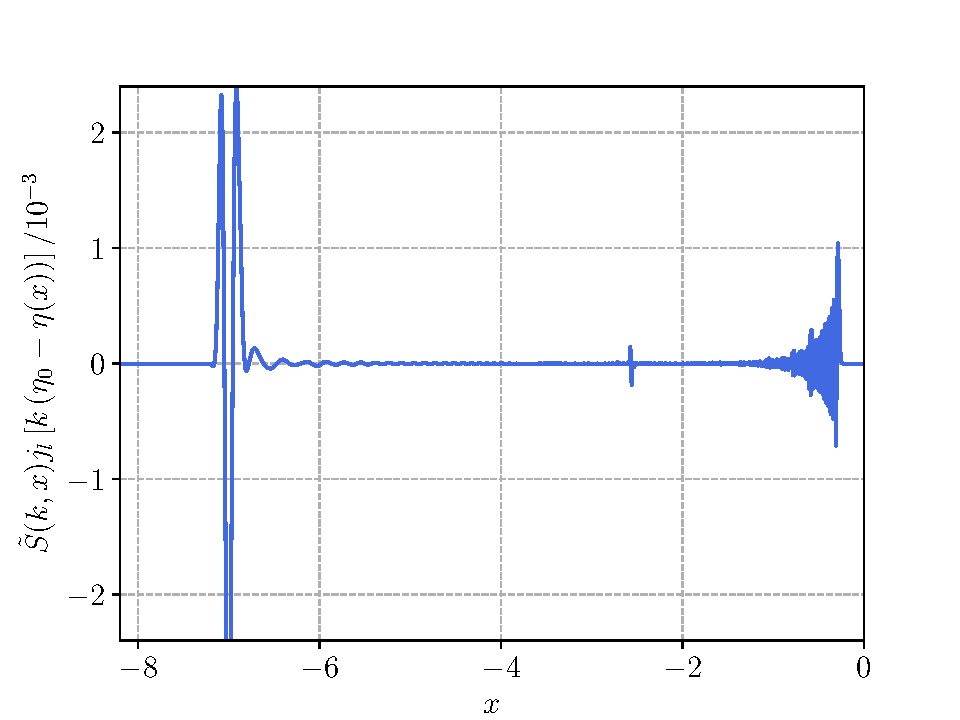
\includegraphics[width = 0.9\textwidth]{callin.pdf}
    \caption{The integrand of the transfer function $\Theta_\ell(x,k)$ plotted as a function of $x$ for $\ell = 100$ and $k = 340H_0/c$.}
    \label{fig: callin}
\end{figure}
We observe that the results do behave in a similar fashion to the results of Callin even though the amplitudes of the peaks dont quite match. In addition, we observe some noise around $x \approx -2.5$. 

\subsection{The Transfer Function}
We proceed by plotting the transfer function for 6 different values of $\ell$. The results of this is seen in figure \ref{fig: transfer}.
\begin{figure}
    \centering
    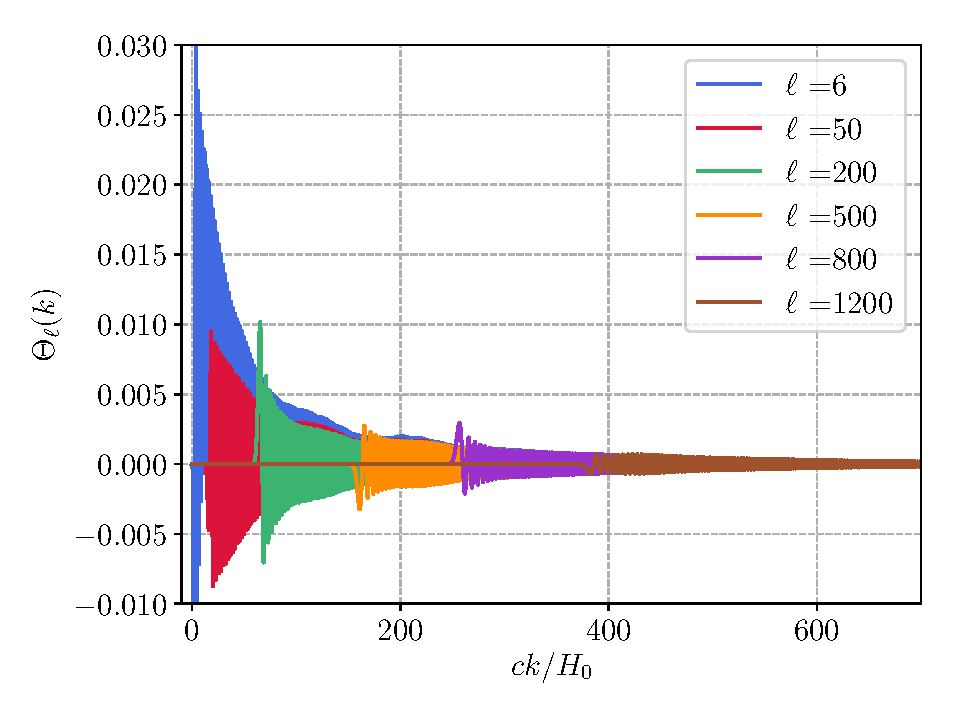
\includegraphics[width = 0.9\textwidth]{transfer.pdf}
    \caption{The transfer function plotted as a function of $k$ for 6 different values of $\ell$.}
    \label{fig: transfer}
\end{figure}
We observe that different values of $\ell$ for the transfer function correspond to different scales in Fourier space. For small values of $\ell$ we see that large scales dominate the transfer function, and correspondingly for high $\ell$'s, small scales provide the significant contribution. It also appears as the the spread of the transfer function increases as a function of $\ell$. The $\ell = 6$ scale has a much higher amplitude than the other $\ell$'s which is a bit worrying. This might suggest that something breaks down for low $\ell$'s in our code.

In order to better be able to study how the actual contribution of the transfer function to the $C_\ell$'s, we will plot the spectrum integrand $\Theta_\ell (k)^2/k$. The results of this is seen in figure \ref{fig: integrand}
\begin{figure}
    \centering
    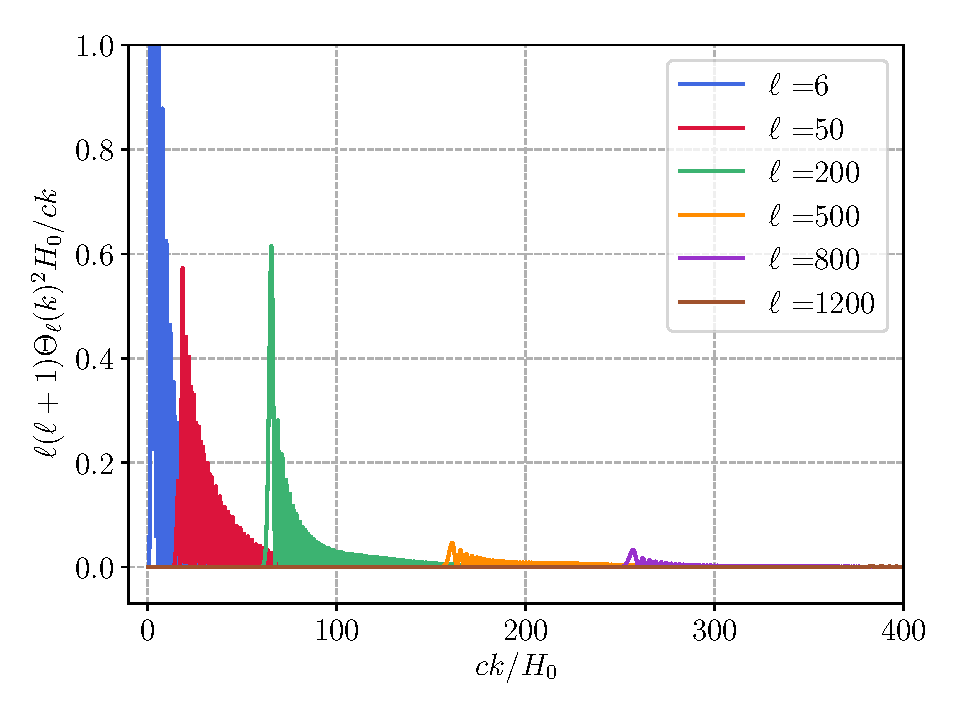
\includegraphics[width = 0.9\textwidth]{integrand.pdf}
    \caption{The spectrum integrand plotted as a function of $k$ for 6 different values of $\ell$. The integrand is multiplied with $\ell(\ell +1)$ to increase the amplitude of the large $\ell$'s.}
    \label{fig: integrand}
\end{figure}
We again observe that $\ell = 6$ is much larger than the other scales, perhaps indicating a bug in the code. This plot is better at indicating which specific values of $k$ the different $\ell$ integrands contributes to. Out of the $6$ different scales, we see that the largest contribution occurs around $\ell \approx 200$ (ignoring the unusually large $\ell = 6$ contribution). 

\subsection{The Angular Power Spectrum}
Now that we have studied the functions from which the CMB power spectrum is constructed, we are ready to plot the spectrum. 
\subsubsection{$\Lambda$CDM}
Using the cosmological parameters of the $\Lambda$CDM model, we get the following power spectrum seen in figure \ref{fig: lcdm}.
\begin{figure}
    \centering
    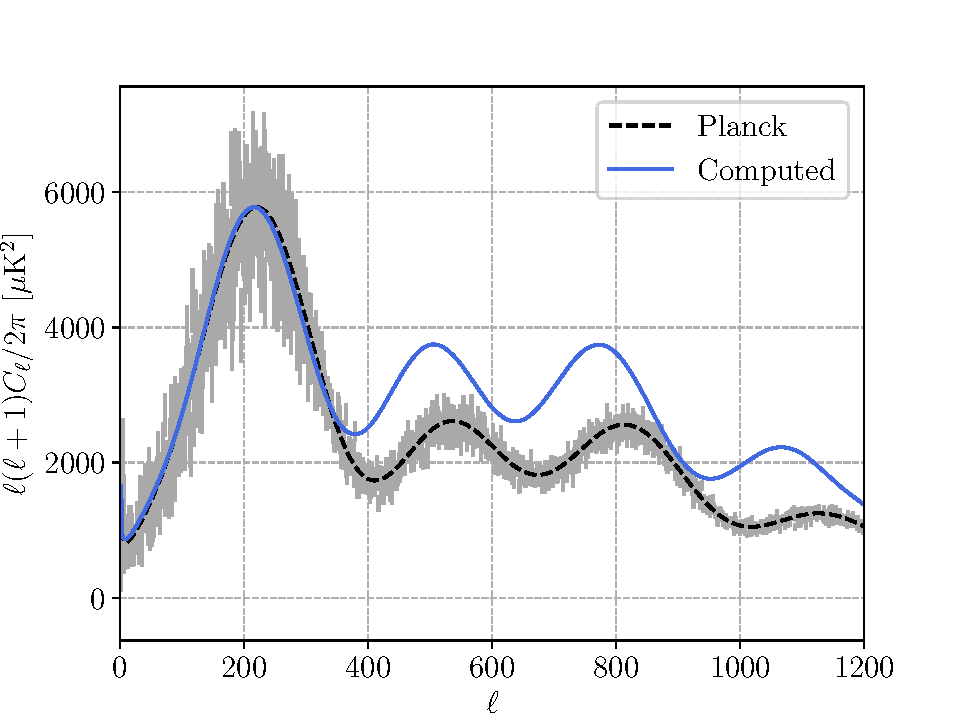
\includegraphics[width = 0.9\textwidth]{cl_lcdm.pdf}
    \caption{The CMB power spectrum as a function of $\ell$, computed using $\Lambda$CDM parameters along with the observed power spectrum from Planck along with error bars displaying the uncertainty. The computed power spectrum is normalized so that the first peak corresponds to the maxima from Planck at 5775 $\mu$K$^2$.}
    \label{fig: lcdm}
\end{figure}
We see that the overall shape and behavior of the computed power spectrum follows the Planck data well. The second and third peaks are however too high. The high amplitude for low $\ell$'s found in both the transfer function and the spectral integrand is visible as we see the amplitude of $\ell = 2$ being quite high. It is however within the uncertainties of the Planck observations. The biggest factor to why the 2nd, 3rd and 4th peak deviate from the observed peaks are likely because of our simplified model where we have ignored neutrinos and polarization. 

\subsubsection{Parameter estimation}
In order to understand the behaviour of the power spectrum better we will now alter the cosmological parameters. This will allow us to better understand the role of the parameters. In figure \ref{fig: vary}, we have slightly altered the paramters $\Omega_b$, $\Omega_m$, $n$ and $h$ one at a time. A discussion around the results can be found in the captions of each figure.

\begin{figure}
\makebox[\textwidth][c]{
  \begin{subfigure}[t]{0.7\textwidth}
    \centering
    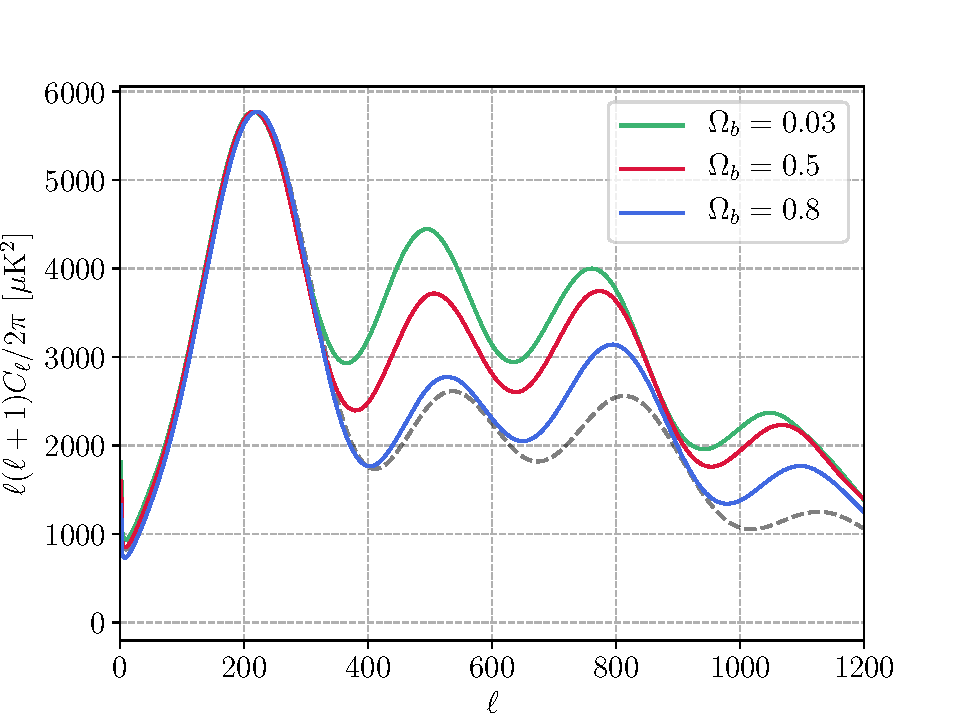
\includegraphics[width=0.9\textwidth]{cl_b.pdf} 
    \caption{The power spectrum $C_\ell$ when varying the fraction of baryonic matter $\Omega_b$. We observe that any change in $\Omega_b$ results in a significant change to the entire spectrum. Increasing the fraction seems to lower the 2nd, 3rd and 4th peak significantly, but with a larger decrease on the 2nd peak. It should be noted that the first peak is fixed due to the normalization with Planck data. The opposite is true when increasing the fraction, where the entire spectrum increases in strength, with the largest increase in the 2nd peak.} 
    \label{fig: 1a} 
  \end{subfigure}%% 
  \begin{subfigure}[t]{0.7\textwidth}
    \centering
    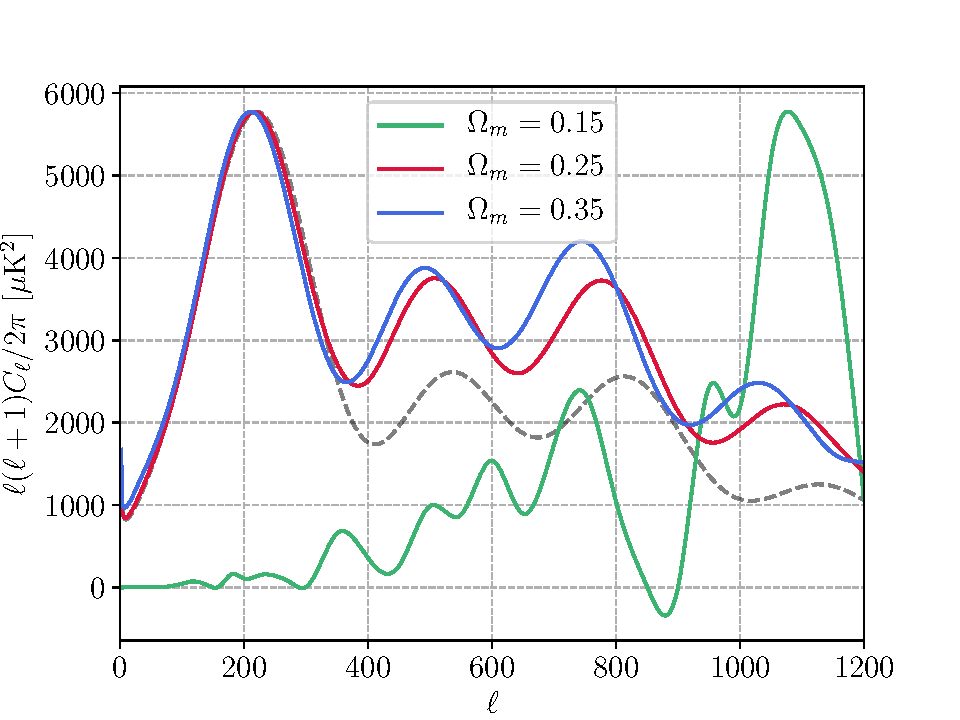
\includegraphics[width=0.9\textwidth]{cl_m.pdf} 
    \caption{The power spectrum $C_\ell$ when varying the fraction of dark matter $\Omega_m$. We see that by increasing the fraction of dark matter in the Universe the overall strength of the spectrum increases with the biggest impact on the 3rd peak. By decreasing the dark matter the opposite happens where the 3rd and 4th peaks are a bit lower. We also see that for very low dark matter fractions, the Universe breaks down which is expected as dark matter is essential for structure formation.} 
    \label{fig: 1b} 
  \end{subfigure} 
  }
  \makebox[\textwidth][c]{
  \begin{subfigure}[t]{0.7\textwidth}
    \centering
    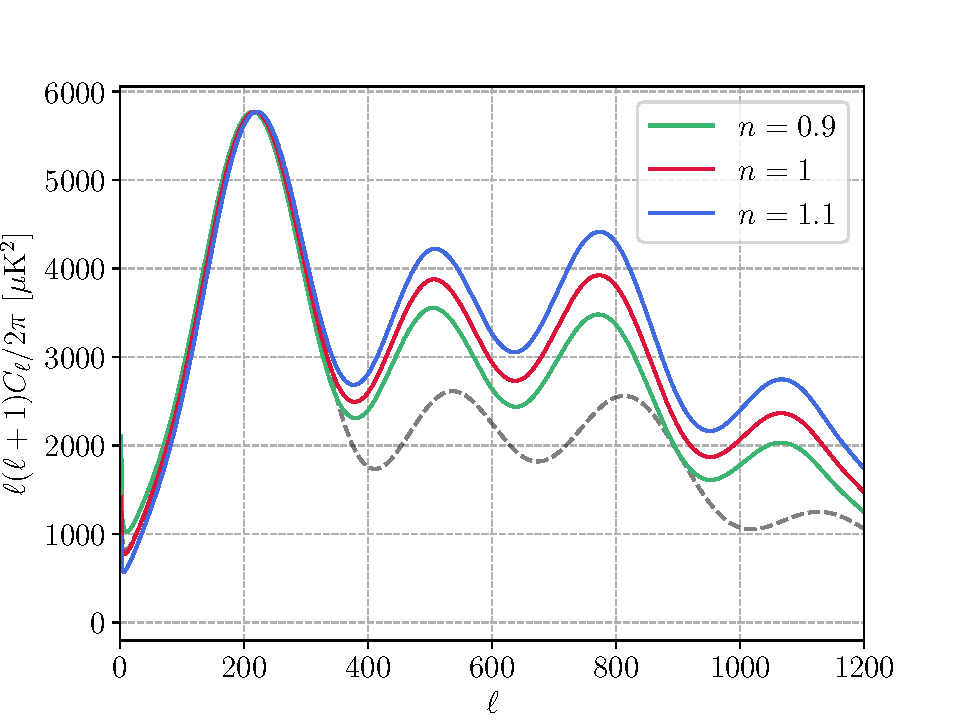
\includegraphics[width=0.9\textwidth]{cl_n.pdf} 
    \caption{The power spectrum $C_\ell$ when varying scalar spectral index $n$. We observe that increasing $n$ results in a overall higher strength to the power spectrum. When lowering $n$ the strength of the spectrum decreases. This is expected from the definition of the power spectrum where $n$ works as a scaling of the the $C_\ell$'s with $n>1$ increasing the overall strength, while $n<1$ decreases the spectrum.} 
    \label{fig: 1c} 
  \end{subfigure}%%
  \begin{subfigure}[t]{0.7\textwidth}
    \centering
    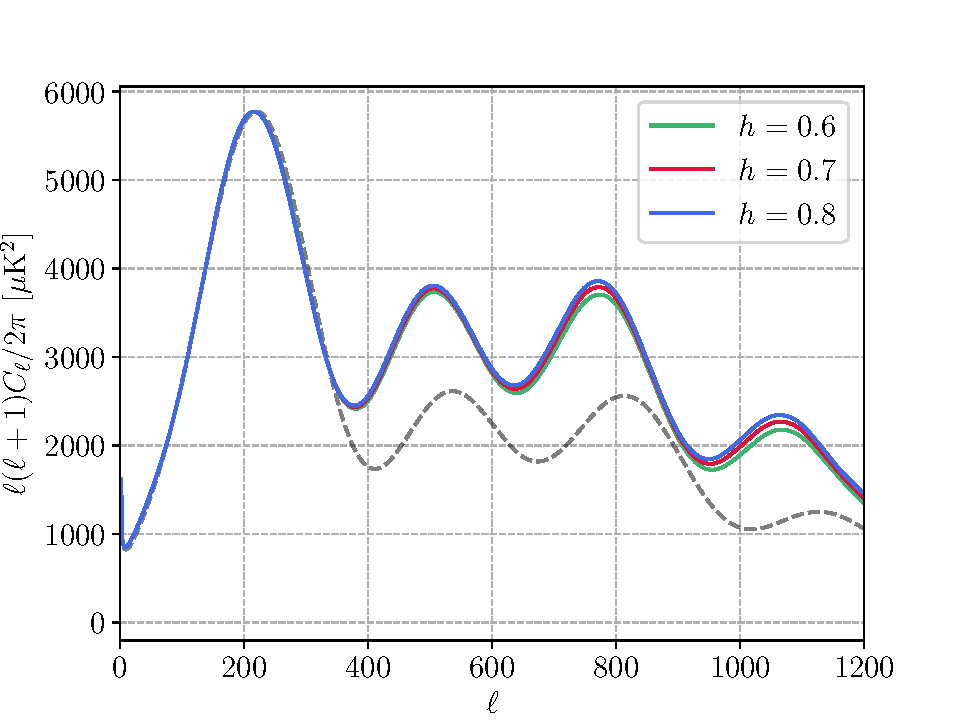
\includegraphics[width=0.9\textwidth]{cl_h.pdf} 
    \caption{The power spectrum $C_\ell$ when varying scaling factor in the Hubble parameter $h$. We see that the significance of changing $h$ is minimal compared to varying the other parameters. The little change we observe is a slight increase to the spectrum when $h$ is increase, and a slight decrease when lowering $h$. We do see that the effect seems to be increasing with the number of peaks as the 4th peak changes much more relative to the 2nd, meaning that the entire spectrum is slightly shifted.} 
    \label{fig: 1d} 
  \end{subfigure} 
  }
  \caption{Figures showing the effects of changing the cosmological parameters. 3 parameters changes to the default parameters are shown where we go slighly above and belove to see the effects the individual parameter has on the power spectrum.}
  \label{fig: vary} 
\end{figure}

\subsubsection{Best-fit parameters}
The observed effects during the parameter varying can motivate our decision on which parameters we should vary and to what extent in order to reach a best-fit. We have chosen to altered the parameters "by hand" rather than doing it through numerical means. One example of a numerical solution to finding best-fit parameters could be Monte Carlo Markov chain algorithms with Metropolis acceptance. Doing so would have given us the best fit parameters, however duo to time constraints we have chose to use the "by hand" method where we changed one parameter at a time until we found a "best" fit. The results of the best-fit estimation is seen in figure \ref{fig: best}. The chosen parameters can be seen in table \ref{tab: best}. 

The best-fit CMB power spectrum does fit the observed Planck data much better than the $\Lambda$CDM parameters. However, we did have to nearly double the assumed baryon content of the universe along with significantly decreasing the dark matter content. These drastic changes would likely not have been necessary if we had included neutrinos and polarization. Our best-fit model is therefore not a realistic model, but it serves the purpose of demonstrating how the power spectrum depends on the parameters. 

\begin{figure}
    \centering
    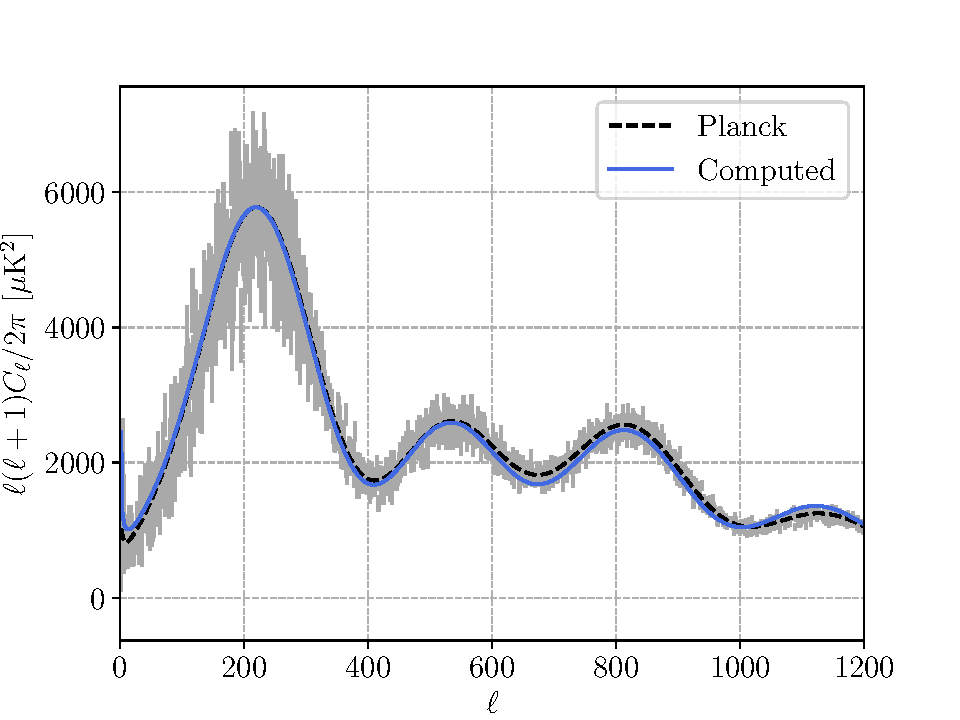
\includegraphics[width = 0.9\textwidth]{cl_best.pdf}
    \caption{The best fit parameter estimation to the CMB power spectrum, plotted as a function of $\ell$. }
    \label{fig: best}
\end{figure}

\begin{table}
\caption{Best-fit parameters found through "by hand" parameter estimation, along with the $\Lambda$CDM parameters.}
\label{tab: best}
\begin{tabular}{lllll}
\hline
\hline
&$\Omega_b \qquad\qquad$ & $\Omega_m \qquad\qquad$ & $n \qquad\qquad$ & $h$ \\ \hline
Best-fit $\qquad$&0.0720      & 0.2000        & 1.2000 & 0.6000 \\
$\Lambda$CDM $\qquad$& 0.0486 & 0.2589 & 0.9667 & 0.6774\\
\hline
\end{tabular}
\end{table}

\section{Conclusion}
To conclude the discussion; the CMB power spectrum is highly parameter dependant. Changing certain parameters such as the baryon and dark matter fraction in the Universe results in significant changes to the spectrum. The best-fit estimate resembles the observed Planck spectrum, but is not very realistic as a result of large changes to well established parameters. Fine tuning the parameters did however give insight to how the different parameters affect the power spectrum. Including polarization would likely fix some, if not most of the encountered errors.

It is time to conclude our 4 milestone long project. It has been a very enjoyable project. The Cosmic microwave background is the pillar of which modern cosmology is built upon, and understanding and even computing it has been very educational.

\bibliography{references}{}
\bibliographystyle{plain}
\end{document}